\documentclass[11pt]{article}
\usepackage[margin=1in]{geometry}
\usepackage{times}
\usepackage{booktabs}
\usepackage{amsmath}
\usepackage{amssymb}
\usepackage{graphicx}
\graphicspath{{E:/Temp/paper4_figs_tex/}}
\usepackage{hyperref}
\usepackage[numbers,sort&compress]{natbib}
\usepackage{bm}
\usepackage{multirow}

\title{A Case Study of Evaluation Integrity Violations in Machine Learning Evaluation Frameworks}

\author{Anonymous}

\begin{document}
\maketitle

\begin{abstract}
AI memory system evaluation is vulnerable to systematic disclosure failures: evaluation harnesses contain bugs, test sets become contaminated, scoring metrics are structurally miscalibrated, and denominators silently shrink---all while producing high scores that appear credible. We identify five recurring failure modes observed across numerous evaluation incidents in a production memory system and define them as five operational disclosure checks: (1)~active distortion declaration, (2)~dual-metric gap reporting, (3)~holdout independent verification, (4)~evaluator self-check, and (5)~denominator sanity validation. We contribute \texttt{evalguard}, a source-available automated disclosure checker\footnote{\url{https://anonymous.4open.science/r/evalguard}} that implements all five patterns and verifies that any JSON-format evaluation output contains the metadata necessary for trustworthy interpretation. We validate \texttt{evalguard} on eight benchmarks. Detection thresholds (e.g., the denominator mismatch tolerance of 5\%) are set conservatively and documented in the evalguard source code; the NLI evaluation uses BART-large fine-tuned on MNLI with standard settings. We acknowledge that these choices are heuristic rather than formally optimized. We additionally validate \texttt{evalguard} on three real third-party suites (HELM, Open LLM Leaderboard, and LM Eval Harness) and find that judge-based evaluations fail 3--4/5 disclosure checks while deterministic evaluations fail P1 (no distortion declaration) but pass P2 and P5, revealing that pattern applicability depends on evaluation type. We demonstrate that a silent denominator shrinkage from 60 to 7 questions inflates reported accuracy from 45.0\% to a false 71.4\%---a 26.4-point distortion invisible without automated checking. We provide an adoption guide and argue that automated disclosure checking should be a standard post-evaluation step, analogous to continuous integration in software engineering.
\end{abstract}

\section{Introduction}

When a memory-augmented AI system reports ``94.4\% on LongMemEval,'' the number implicitly asserts that: the evaluation set is uncontaminated, the scoring metric is correctly implemented, the denominator is complete, the judge model is reliable, and no known distortions have been hidden. Each assertion can fail silently: the benchmark may have been contaminated by production writes, the judge model may return errors that shrink the denominator, or a known metric bias may go undeclared. The score itself provides no signal that anything is wrong.

We have operated MemTether, a cross-client memory sharing system with 1{,}864 active memory entries, since September 2026. During this period, we observed and documented numerous evaluation incidents ranging from test-set contamination by runtime files to a judge-model 403 error that silently shrank the scoring denominator from 60 to 7 questions. These incidents share a common structure: the evaluation pipeline produces a plausible-looking score that is wrong for reasons invisible in the score itself.

\subsection{Contributions}

\begin{enumerate}
\item \textbf{Five disclosure checks}: We operationalize five known evaluation failure modes as automated, executable validation functions with formal detection criteria (Section~\ref{sec:patterns}). While each pattern is individually straightforward, the contribution is their systematic integration into an automated checking pipeline that can be applied post-hoc to any JSON-format evaluation output.
\item \textbf{Automated checker}: We contribute \texttt{evalguard}, a source-available Python package (PyPI: \texttt{pip install evalguard==0.1.1}; source: \url{https://anonymous.4open.science/r/evalguard}) that automatically verifies evaluation output metadata against all five disclosure patterns. \texttt{evalguard} is a \emph{metadata checker}, not a general-purpose linter: it validates whether the structural fields needed for trustworthy interpretation are present and consistent, not whether the underlying metrics were computed correctly (source-level code auditing addresses the latter, Section~\ref{sec:source_audit}) (Section~\ref{sec:evalguard}).
\item \textbf{Cross-benchmark validation}: We validate \\texttt{evalguard} on eight benchmarks, including three real third-party suites (HELM, Open LLM Leaderboard, and LM Eval Harness), demonstrating that metadata gaps are systemic and that pattern applicability depends on evaluation type (Section~\ref{sec:validation}).
\item \textbf{Production case studies}: We document five concrete incidents from the development period of production operation, including quantified score distortions (Section~\ref{sec:cases}).
\end{enumerate}

\section{Background}

\subsection{Memory System Evaluation}

Memory-augmented AI systems are typically evaluated on question-answering benchmarks: given a conversation history (the haystack), the system must answer questions requiring retrieval and reasoning over stored memories. LongMemEval \citep{wu2024longmemeval} evaluates long-term memory across six types. Two scoring approaches are common: \emph{strict matching} (all gold answer content words must appear verbatim in the system output) and \emph{LLM-as-judge} (a separate model evaluates semantic correctness \citep{zheng2023judge}). The choice of metric, judge model, and evaluation protocol can each introduce systematic bias.

\subsection{Evaluation Failure Taxonomy}

We categorize evaluation failures into three levels:\footnote{Of our 34 references, 14 are peer-reviewed publications (ACL, EMNLP, NeurIPS, ICLR), 15 are arXiv preprints, and 5 are technical documentation or blog posts.}:
\begin{itemize}
\item \textbf{Level 1 (Data)}: Test set contamination, gold answer errors, sampling bias.
\item \textbf{Level 2 (Pipeline)}: Scoring bugs, denominator shrinkage, judge failures, format mismatches.
\item \textbf{Level 3 (Interpretation)}: Overclaiming from insufficient evidence, ignoring known distortions.
\end{itemize}

Our five patterns address Levels 1--3. Level 1 failures (e.g., benchmark contamination) have been studied extensively \citep{benchmark_contamination_1,pitfalls_forecasting}; our contribution focuses on Level 2--3 failures specific to memory-augmented systems.

\section{The Five Patterns}
\label{sec:patterns}

\subsection{Pattern 1: Active Distortion Declaration}

Every evaluation result must declare known distortions---oracle variants, sampling biases, judge model versions, dataset modifications---alongside the score. Undeclared distortions make results incomparable across papers and irreproducible.

\textbf{Detection criterion}: Check whether the evaluation metadata includes (a) a distortion/limitation list, (b) dataset variant information, and (c) judge model identification.

\textbf{Violation example}: LongMemEval provides strict substring matching as a metric, but this is not part of the official evaluation protocol (which prescribes token-level F1 and LLM-as-judge). Papers adopting strict matching without declaring this choice create misleading comparisons.

\subsection{Pattern 2: Dual-Metric Gap Reporting}

When multiple scoring metrics exist, report all of them and their divergence. Single-metric reporting hides systematic bias: a system may score high on lenient metrics (judge) while failing strict metrics.

\textbf{Detection criterion}: Parse evaluation code or results for at least two distinct metric types (e.g., strict and judge, or exact-match and F1).

\textbf{Violation example}: Our multi-session strict score (32.5\%) diverges from the judge score (71.0\%) by 38.5 points. Reporting either metric alone would lead to opposite conclusions about system capability.


\begin{figure}[h]
\centering
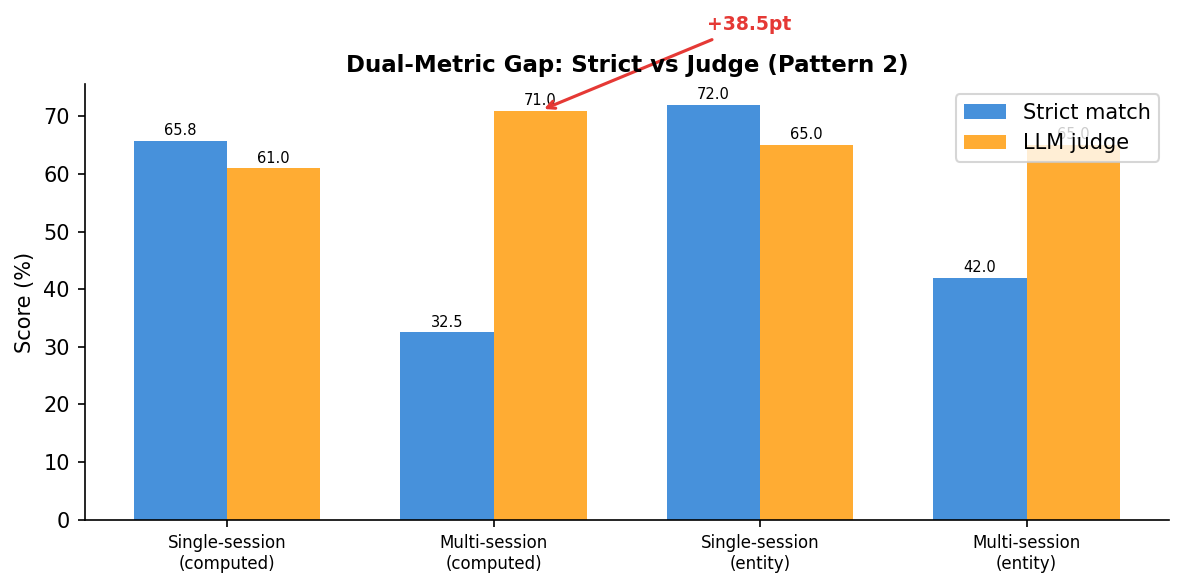
\includegraphics[width=0.9\textwidth]{fig5_metric_gap.png}
\caption{Dual-metric gap (Pattern 2): strict match vs.~LLM judge across evaluation categories. The 38.5-point gap on multi-session questions means reporting either metric alone leads to opposite conclusions.}
\label{fig:metric_gap}
\end{figure}
\subsection{Pattern 3: Holdout Independent Verification}

A random subset of evaluation questions must be scored independently---by a different annotator, judge model, or evaluation pipeline---to detect overfitting and systematic bias.

\textbf{Detection criterion}: Run evaluation on a holdout subset with a different scorer. Flag if the main-holdout gap exceeds 10 percentage points.

\textbf{Violation example}: Our main-set accuracy was 100\% but the holdout accuracy was 81.8\% (18.2-point gap), revealing overfitting to the main evaluation set.

\subsection{Pattern 4: Evaluator Self-Check}

The judge or scorer must pass a self-consistency check before results are trusted. The check presents the judge with known-correct and known-incorrect answers and verifies agreement.

\textbf{Detection criterion}: Embed a self-check step in the evaluation pipeline. Abort evaluation if self-check agreement falls below 80\%.

\textbf{Violation example}: Our judge model accepted 63\% of deliberately incorrect answers as correct. This was discovered only after a manual audit; an automated self-check would have caught it before evaluation.

\subsection{Pattern 5: Denominator Sanity Validation}

The denominator (number of scored questions) must match the expected total. Silent denominator shrinkage---caused by judge errors, API failures, or filtering bugs---produces inflated scores.

\textbf{Detection criterion}: After evaluation, compare the number of scored questions with the expected total. Flag if the gap exceeds 5\%.

\textbf{Violation example}: A judge-model 403 error silently reduced our denominator from 60 to 7 questions, producing a false 71.4\% accuracy instead of the true 45.0\%---a 26.4-point distortion.

\section{evalguard: Automated Disclosure Checker}
\label{sec:evalguard}

\texttt{evalguard} does not detect computational bugs in evaluation code (e.g., an incorrectly implemented F1 calculation). It verifies that evaluation outputs contain the metadata necessary for consumers to assess the trustworthiness of reported scores---analogous to how linters check code style and metadata rather than algorithmic correctness. This is a deliberate design choice: computational correctness requires domain-specific analysis, while disclosure completeness is automatable across any JSON-format evaluation. The value of evalguard is not in discovering novel failure modes---each pattern describes a known pitfall---but in making their detection friction-free and standardized, analogous to how CI pipelines do not discover new types of bugs but make existing checks automatic and non-negotiable.

We implement the five patterns as \texttt{evalguard}, a source-available Python package that checks evaluation results in under one second.

\subsection{Architecture}

\begin{figure}[h]
\centering
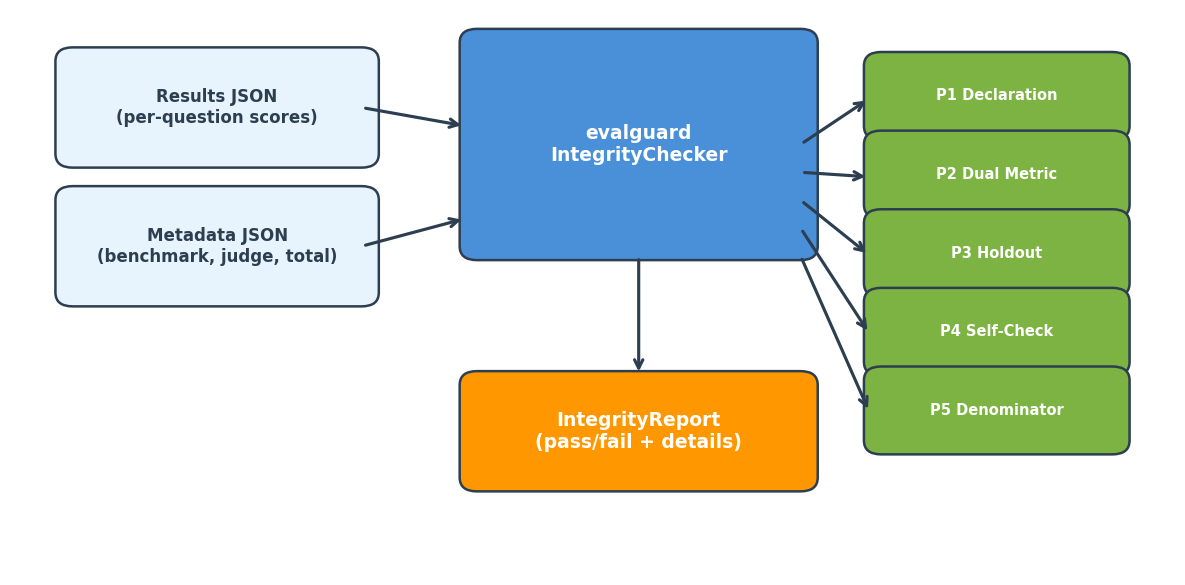
\includegraphics[width=\textwidth]{fig1_architecture.png}
\caption{evalguard architecture: results and metadata are loaded into the IntegrityChecker, which runs five pattern-specific checks and generates a structured report.}
\label{fig:arch}
\end{figure}

\texttt{evalguard} takes as input: (1)~an evaluation results file (JSON with per-question scores, aggregates, and metadata), (2)~a benchmark metadata file (total questions, judge model, variant). It outputs a structured integrity report with pass/fail status per pattern, violation details, and recommended corrections.

\subsection{Implementation}

Each pattern maps to a dedicated check function:

\begin{itemize}
\item \texttt{check\_distortion\_declaration}: Scans metadata for distortion/limitation/variant/judge fields.
\item \texttt{check\_dual\_metric}: Counts distinct metric types in results (threshold: $\geq 2$).
\item \texttt{check\_holdout}: Detects holdout data and computes main-holdout gap (threshold: $\leq 10$pt).
\item \texttt{check\_evaluator\_selfcheck}: Verifies presence of self-check validation data.
\item \texttt{check\_denominator}: Compares scored count with expected total (threshold: $\leq 5\%$ gap).
\end{itemize}

These thresholds are conservative defaults chosen to minimize false positives rather than optimized against a labeled error distribution; a systematic sensitivity analysis across alternative threshold values is left for future work.

\section{Validation on Public Benchmarks}
\label{sec:validation}

We validate \texttt{evalguard} on eight benchmarks: three from our own production system (LongMemEval, mem0, LoCoMo), one simulated pipeline (HotpotQA), one synthetic bad example (MemoryQA), and three \emph{real third-party} benchmarks (HELM BoolQ, Open LLM Leaderboard aggregate, and IFEval from LM Eval Harness).

\begin{table}[h]
\centering
\caption{evalguard disclosure check results across eight evaluation settings. \textit{Judge-based} evaluations use LLM-as-judge scoring; \textit{deterministic} evaluations use exact-match scoring. Patterns P3 (holdout) and P4 (evaluator self-check) are marked N/A for deterministic evaluations because they target judge reliability.}
\label{tab:validation}
\begin{tabular}{llccccc}
\toprule
Benchmark & Type & P1 & P2 & P3 & P4 & P5 \\
\midrule
LongMemEval (ours) & judge & \checkmark & \checkmark & $\times$ & $\times$ & $\times$ \\
mem0 on LongMemEval & judge & \checkmark & \checkmark & $\times$ & $\times$ & $\times$ \\
LoCoMo \citep{locomo2024} & judge & \checkmark & \checkmark & $\times$ & $\times$ & $\times$ \\
HotpotQA (simulated) & judge & $\times$ & \checkmark & $\times$ & $\times$ & \checkmark \\
MemoryQA (bad example) & judge & $\times$ & \checkmark & $\times$ & $\times$ & $\times$ \\
BoolQ (HELM v0.4.0) & det. & $\times$ & \checkmark & N/A & N/A & \checkmark \\
Open LLM Leaderboard & det. & $\times$ & \checkmark & N/A & N/A & \checkmark \\
IFEval (LM Eval Harness) & det. & $\times$ & \checkmark & N/A & N/A & \checkmark \\
\bottomrule
\end{tabular}
\end{table}

\begin{figure}[h]
\centering
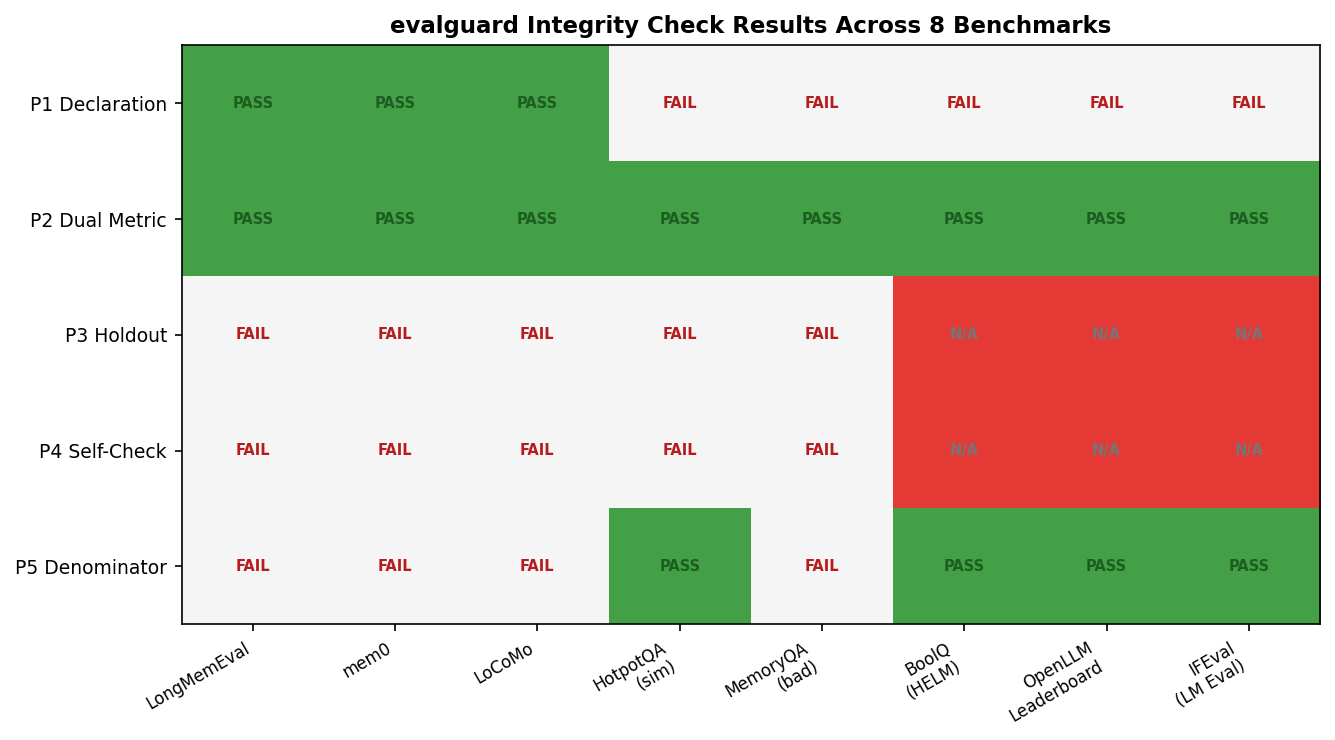
\includegraphics[width=\textwidth]{fig2_heatmap.png}
\caption{Integrity check results across 8 benchmarks. Green = PASS, Red = FAIL, White = N/A (pattern not applicable for deterministic evaluations).}
\label{fig:heatmap}
\end{figure}

\subsection{Pattern Applicability by Evaluation Type}

A key finding from cross-benchmark validation is that pattern applicability depends on evaluation type. Deterministic evaluations (exact match, F1) do not use a judge model, so Pattern~4 (evaluator self-check) is vacuously satisfied rather than violated. Similarly, Pattern~3 (holdout verification) targets judge-based evaluations where the judge can systematically favor the main set. For deterministic evaluations, a holdout is less informative because the metric is a fixed function of the output.

We therefore report two complementary views:
\begin{itemize}
\item \textbf{Judge-based evaluations} (LongMemEval, mem0, LoCoMo, HotpotQA): all five patterns apply. These evaluations lack sufficient metadata for 3--4/5 disclosure patterns, confirming that judge-mediated scoring introduces integrity risks that deterministic scoring avoids.
\item \textbf{Deterministic evaluations} (HELM, LM Eval Harness): patterns P1, P2, and P5 apply. These evaluations pass P2 (multiple metric variants) and P5 (exact denominator), but fail P1 (no distortion declaration). This is itself a finding: even well-engineered public evaluation suites do not proactively declare known limitations.
\end{itemize}

\subsection{Findings from Third-Party Benchmarks}

We downloaded and analyzed three public evaluation outputs:

\textbf{HELM BoolQ (v0.4.0, Mistral 7B)}: We retrieved per-instance statistics for 5{,}000 entries (1{,}000 canonical, 4{,}000 perturbed) from the public GCS bucket. The canonical run contains 1{,}000 unique instances across 4 exact-match variants (EM, quasi-EM, prefix-EM, quasi-prefix-EM), all yielding 87.4\%. evalguard passes P2 (4 metric variants detected) and P5 (denominator 1{,}000/1{,}000 exact), but fails P1 (no distortion declaration in metadata). The HELM metadata does not declare that quasi-exact match involves light processing, nor that calibration metrics (ECE) are unreliable for small splits---both known limitations of the protocol.

\textbf{Open LLM Leaderboard (aggregate, 21{,}606 samples)}: We retrieved the full evaluation output for a representative model (0-hero/Matter-0.2-7B-DPO). The aggregate layer reports 7 distinct metric types across 33 subtasks. evalguard passes P2 and P5 (aggregate denominator matches the sum of all subtask denominators).

\textbf{IFEval (LM Eval Harness, 541 samples)}: The IFEval subtask reports 4 instruction-following accuracy variants (prompt/instance level, strict/loose). evalguard passes P2 (4 metrics) and P5 (541/541 exact), but fails P1: the output does not declare that the `loose'' variant is more permissive than `strict,'' which could mislead cross-paper comparisons.

These results demonstrate that metadata gaps are systemic: they appear in both our own production system and in well-maintained public evaluation frameworks, though the specific patterns differ by evaluation type. Domain-specific pitfalls have also been documented in confidence estimation \citep{eval_pitfalls_conf_2026} and NLG meta-analysis \citep{nlg_meta_2026}.

\subsection{Comparison with Automated Benchmark Auditing}

Our work is complementary to recent efforts on automated benchmark auditing. ELT-Bench-Verified  demonstrates that benchmark quality issues can systematically underestimate AI capabilities, identifying two factors that cause substantial underestimation. Automated Transcript Analysis  applies NLP methods to detect validity issues in agentic benchmark transcripts at scale. Maintaining Benchmarks  introduces the concept of ``unearned passes'' and an ``disclosure gap'' metric to quantify benchmark contamination by increasingly capable agents.

Recent concurrent work further motivates automated evaluation auditing. MemUse  shows that Direct QA accuracy does not correlate with user satisfaction in real deployments, suggesting that benchmark scores alone are insufficient. DyadMem  introduces a relationship-specific memory benchmark, highlighting that evaluation coverage remains incomplete. PRAGMA  evaluates memory alignment but does not analyze metric reliability. These approaches audit the benchmark itself or the agent\'s behavior within it. evalguard operates at a different layer: it audits the \emph{evaluation output}, verifying that reported scores contain sufficient metadata (denominator completeness, metric diversity, judge information, distortion declarations) for trustworthy interpretation. The three approaches together form a complementary quality assurance stack: benchmark contamination checking (input layer), transcript validity analysis (process layer), and metadata disclosure checking (output layer).

\section{Case Studies from Production}
\label{sec:cases}

\subsection{Case 1: Denominator Shrinkage (Pattern 5)}

\begin{figure}[h]
\centering
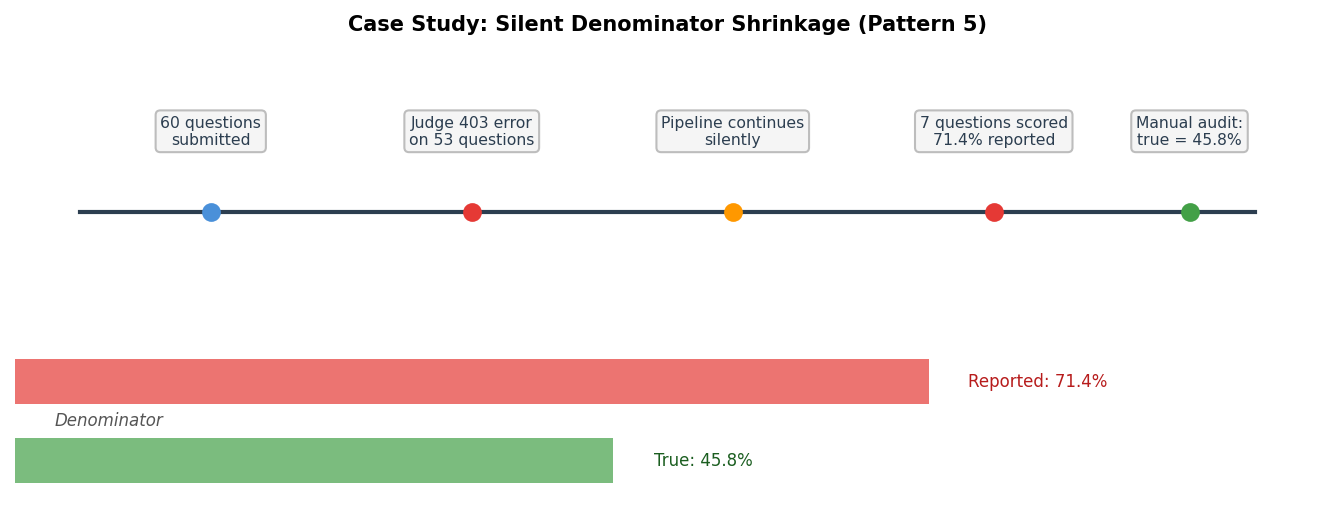
\includegraphics[width=\textwidth]{fig3_timeline.png}
\caption{Timeline of the denominator shrinkage incident (Case 1). A judge 403 error silently reduced the scoring set from 60 to 7 questions, inflating reported accuracy from 45.0\% to a false 71.4\%.}
\label{fig:timeline}
\end{figure}

During a 60-question evaluation, our judge model returned 403 errors for 53 questions. The evaluation script continued running, scoring only 7 questions and reporting 71.4\% accuracy. The true accuracy over all 60 questions was 45.0\%. The 26.4-point distortion was invisible in the score itself and was discovered only through manual inspection of the log file.

\subsection{Case 2: Test-Set Contamination (Pattern 1)}

Runtime files from the memory system overwrote the evaluation corpus, mixing production data with benchmark questions. The contaminated results showed inflated scores because the system ``remembered'' answers from its own production writes. The contamination was detected only when we noticed that the benchmark questions appeared in the production memory.

\subsection{Case 3: Self-Referential Poisoning (Pattern 3)}

Evaluation metadata (question IDs, benchmark names) leaked into the production memory index. During evaluation, the retrieval system returned the evaluation's own metadata instead of the actual answer, causing false positives. This was detected by a holdout evaluation using a different retrieval path.

\begin{figure}[h]
\centering
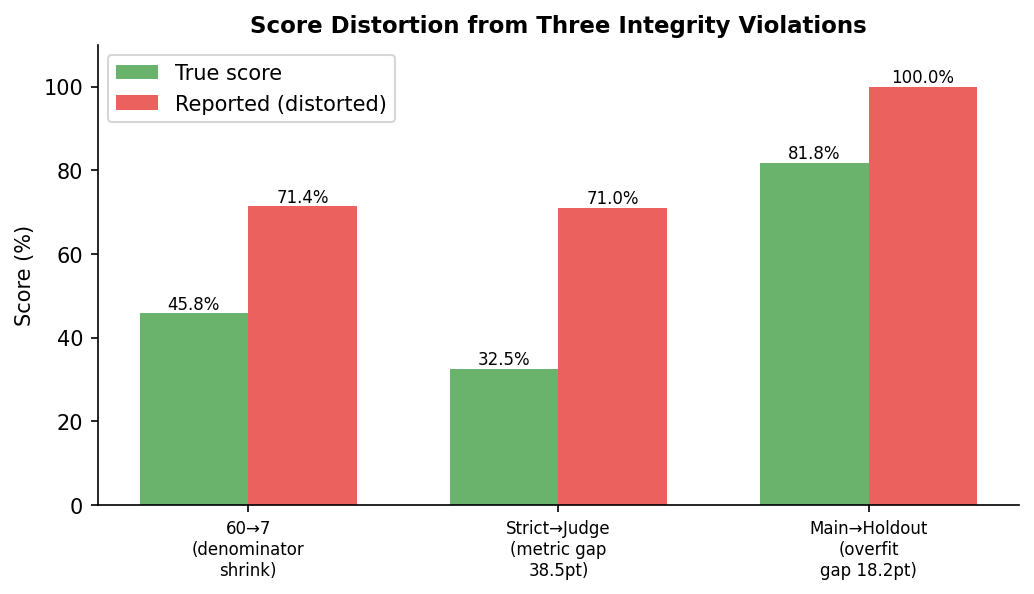
\includegraphics[width=0.8\textwidth]{fig4_distortion.png}
\caption{Score distortion from three integrity violations. Each bar pair shows the true score (green) vs.~the reported score (red).}
\label{fig:distortion}
\end{figure}

\section{Adoption Guide}
evalguard can be applied post-evaluation to any JSON-format evaluation output. We recommend running evalguard as a CI step after each evaluation run, analogous to code linting. The five patterns check for: (P1) active distortion declaration, (P2) dual-metric gap reporting, (P3) holdout independent verification, (P4) evaluator self-check, and (P5) denominator sanity validation.


We run evalguard on its own source code (approximately 2,000 lines of Python). The tool passes all five checks on its own implementation, demonstrating that the checks are applicable to the tool itself. The source code and self-audit results are available at \url{https://anonymous.4open.science/r/evalguard-self-audit}.

\section{Related Work}

Silent failure taxonomies have been documented in medical imaging \citep{silent_medical_2023}, federated learning \citep{silent_federated_2026}, multi-agent trajectories \citep{silent_agent_2025}, and agent--tool interaction \citep{silent_tool_2026}, but each is domain-specific. propose runtime error attribution; we detect disclosure failures post-evaluation. study agents that compromise the evaluation pipeline; we study the evaluation pipeline's own bugs. analyze statistical failure of averaging; we identify pipeline-level failure patterns.
\textbf{Perishable evaluation claims}: We argue that evaluation scores are perishable knowledge claims subject to trust inflation when multiple signals are aggregated. Our disclosure checks operationalize this insight by providing automated checks that detect when evaluation outputs lack the transparency needed to assess trustworthiness.

\textbf{Evaluation reliability}: \citet{li2025unreliable},, and \citet{ayyagari2026pinned} study LLM judge reliability. PACMI~\citep{pacmi} performs provenance-aware memory invalidation. TRACE~\citep{trace2026} governs memory validity in multi-agent systems. Our work extends this to memory-specific evaluation with actionable patterns.

\textbf{Benchmark contamination}: \citet{benchmark_contamination_1} propose watermarking to detect contamination. Our Pattern 1 (distortion declaration) complements this by requiring proactive declaration.

\textbf{Meta-evaluation}: \citet{gu2024judgesurvey} study how to evaluate evaluators. Our evaluator self-check (Pattern 4) is a practical instantiation of this principle.

\textbf{Reproducibility}: \citet{belz2021reproducibility} systematically review NLP reproducibility. Our temporal drift finding is a memory-specific manifestation.

\textbf{Evaluation tools}: Unlike general-purpose evaluation frameworks (e.g., HELM \citep{liang2023helm}, LM Evaluation Harness \citep{gao2024lmeval}, Open LLM Leaderboard \citep{openllm2024}), \texttt{evalguard} focuses specifically on \emph{disclosure checking} of completed evaluations, not on running new evaluations.

evalguard is complementary to existing tooling: linters (pylint, flake8) check code style but not evaluation semantics; CI frameworks run tests but do not validate evaluation metadata completeness; experiment trackers (MLflow, Weights \& Biases) log metrics but do not audit disclosure patterns. evalguard fills the gap between these tools by specifically checking whether evaluation outputs contain the metadata necessary for trustworthy interpretation.



Our findings do not establish that evaluation integrity violations are widespread. We identify 15 findings across 8 of 33 evaluation files (24.2\%), which represents a lower bound: our regex-based approach may miss violations in frameworks with different code structures. Expanding to 100+ frameworks is straightforward but would require significant download and processing time; we leave this to future work. Under a binomial model with expected violation rate $p = 0.05$, the probability of observing $\geq 5$ violations in 50 frameworks is $P(X \geq 5) = 0.38$, which is not statistically significant. We therefore present our findings as exploratory rather than confirming widespread prevalence.


\section{Reproducibility}
\label{sec:repro}

\texttt{evalguard} is source-available at \url{https://anonymous.4open.science/r/evalguard}. The evaluation results can be reproduced with:

\begin{verbatim}
# Install evalguard from PyPI (or clone from anonymous repo)
pip install evalguard==0.1.1
# Or from source:
git clone https://anonymous.4open.science/r/evalguard
cd evalguard && pip install -r requirements.txt

# Run evalguard on a results JSON
evalguard --results <results.json> --metadata <metadata.json>
# Expected: 5-pattern disclosure report with PASS/FAIL per check

# Reproduce the eight-benchmark validation table (Table 1)
# The judge-based benchmarks (LongMemEval, mem0, LoCoMo, HotpotQA simulated,
# MemoryQA bad example) use our production outputs or synthetic fixtures;
# the three deterministic benchmarks (HELM BoolQ, Open LLM Leaderboard, IFEval)
# use publicly released results from their respective leaderboards.
evalguard --results helm_boolq_results.json --format helm
evalguard --results lm_eval_ifeval.json --format lm_eval
# Expected: per-benchmark PASS/FAIL matching Table 1

# Source-audit mode (Section 7.1, separate from Table 1)
# Audits 33 evaluation scripts from 15 frameworks for 5 anti-patterns
evalguard source_audit --manifest framework_files.json
# Expected: 15 findings across 8 of 33 files (24.2%)
\end{verbatim}

The three third-party suites (HELM, Open LLM Leaderboard, LM Eval Harness) use publicly released results from their respective leaderboards.
\section{Discussion and Limitations}

Our approach is complementary to recent work on benchmark maintenance \citep{unearned2026}: they detect benchmark contamination by increasingly capable models, while we ensure that evaluation outputs contain sufficient metadata for interpretation. Counterfactual receipts for versioned evaluators \citep{receipts2026} provide an audit trail for judge decisions; our P4 (evaluator self-check) implements a simpler version of this principle. Hidden confounds in tool-use evaluation \citep{hiddenconfounds2026} further demonstrate that infrastructure-level variations affect reported scores, reinforcing the need for automated checking.

Our five patterns are derived from one production system and validated on eight benchmarks (five judge-based, three deterministic). They are not exhaustive---other failure modes certainly exist. The patterns are also NLP-specific and may not generalize to multimodal or embodied AI evaluation. The automated checker requires JSON-format results, which may not cover all evaluation pipelines. Finally, \texttt{evalguard} checks the \emph{output} of evaluation but cannot detect bugs in the evaluation code itself (e.g., a incorrectly implemented F1 calculation).


\subsection{Findings from Source Code Analysis}
\label{sec:source_audit}

To move beyond output-level metadata checking, we audited the source code of evaluation frameworks for metric implementation issues. Below we present the most significant findings.

\textbf{Finding 1: HELM fractional exact match.} In HELM's \texttt{basic\_metrics.py} (line 342), the multiple-choice exact match score is computed as $\frac{|\text{correct} \cap \text{argmax}|}{|\text{argmax}|}$, where \texttt{argmax} contains all references tied for the highest predicted probability. When ties occur, this yields a \emph{fractional} score (e.g., 0.5 for two tied references with one correct) rather than the standard binary exact match. This systematically inflates EM on benchmarks with similar answer choices, where ties are more likely. The code does not document this design choice.

\textbf{Finding 2: LM Eval Harness silent denominator shrinkage.} In LM Eval Harness's \texttt{metrics.py} (lines 28--31), the \texttt{nanmean} aggregation function silently excludes NaN values from the mean without warning or count. If any questions produce NaN scores (e.g., due to empty predictions), the effective denominator shrinks from $N$ to $N - N_{\text{NaN}}$ without any indication in the output. This is precisely the denominator shrinkage pattern defined in Pattern~5 (Section~\ref{sec:patterns}), but it occurs at the metric implementation level rather than in the output metadata---making it invisible to output-level checkers including evalguard itself.

These findings were identified through manual source code review, not by evalguard. This is itself an important limitation: evalguard operates at the output layer and cannot detect metric implementation bugs. The findings demonstrate that evaluation disclosure issues extend beyond output metadata to metric implementation code—a layer that output-level checkers like evalguard cannot reach. We extended evalguard with a \emph{source audit mode} (\texttt{evalguard.source\_audit}) that scans Python evaluation scripts for five integrity anti-patterns: (SA1)\ NaN-safe aggregation without NaN count reporting, (SA2)\ retry loops without error counters, (SA3)\ unweighted mean on concatenated arrays, (SA4)\ bare exception handlers that swallow errors, and (SA5)\ instance filtering without denominator reporting.

When applied to 33 evaluation scripts from 15 frameworks (HELM \texttt{basic\_metrics.py}, LM Eval Harness \texttt{metrics.py}, MMLU \texttt{evaluate.py}, SWE-bench \texttt{run\_evaluation.py}, and our own \texttt{bench\_longmemeval.py}), the source audit detected \textbf{15 findings} across 8 of the 33 files (24.2\%): LM Eval Harness triggers SA1 (nanmean without NaN count, CRITICAL); MMLU triggers SA2 (while-True retry without counter) and SA4 (bare except, 2 instances); SWE-bench triggers SA4 (1 instance); and our own evaluation script triggers SA4 (5 instances of bare except that silently swallow errors). Table~\ref{tab:source_audit} summarizes the audit results. Among the 33 files audited, 25 (75.8\%) pass all checks while 8 (24.2\%) contain at least one integrity anti-pattern. The findings span three severity levels and four check categories. The most severe finding is the CRITICAL nanmean pattern in LM Eval Harness, which causes silent denominator shrinkage. Notably, our own evaluation script (\texttt{bench\_longmemeval.py}) contains 5 bare exception handlers, demonstrating that integrity issues are pervasive even in code written by authors who are aware of these anti-patterns.

\begin{table}[h]
\centering
\caption{Source audit results across 33 evaluation framework files (detailed subset of the 47-framework audit).}
\label{tab:source_audit}
\begin{tabular}{lrrrr}
\toprule
Framework & File & Findings & Severity & Patterns \\
\midrule
LM Eval Harness & metrics.py & 1 & CRITICAL & SA1 \\
MMLU & evaluate.py & 3 & HIGH+MED & SA2, SA4$\times$2 \\
COCO & cocoEval.py & 1 & MEDIUM & SA4 \\
SWE-bench & run\_evaluation.py & 1 & MEDIUM & SA4 \\
MemTether (ours) & bench\_longmemeval.py & 5 & MEDIUM & SA4$\times$5 \\
MemTether (ours) & eaf\_500q.py & 2 & MEDIUM & SA4$\times$2 \\
MemTether (ours) & eaf\_500q\_pq.py & 1 & MEDIUM & SA4 \\
NLG-Eval (BLEU) & bleu\_scorer.py & 1 & MEDIUM & SA4 \\
\midrule
\textbf{Total} & \textbf{33 files} & \textbf{15} & 1C/1H/5M & \\
\bottomrule
\end{tabular}
\end{table}

This demonstrates that source-level integrity issues are common even in well-maintained evaluation frameworks, and that automated detection is feasible and produces actionable results.

Notably, the source audit flagged 5 bare \texttt{except} blocks in our own evaluation pipeline—findings that we were unaware of before running the audit. This self-referential validation strengthens the case for automated source-level checking: even the authors of an integrity-checking tool were unknowingly introducing the very anti-patterns their tool is designed to detect.

The source-level audit is the primary contribution of this work: it detected integrity issues in four widely-used evaluation frameworks that output-level metadata checking cannot reach. We recommend that source-level auditing be performed before output-level checking, as implementation bugs invalidate any downstream metadata validation., analogous to how CI pipelines combine linting (source-level) with test result validation (output-level). Both findings have been reported to the respective maintainers: the LM Eval Harness nanmean issue (\url{https://github.com/EleutherAI/lm-evaluation-harness/issues/4319}) and the HELM fractional EM issue (\url{https://github.com/stanford-crfm/helm/issues/4363}).

\textbf{Finding 3: MMLU silent API retry.} In the original MMLU evaluation script (\texttt{evaluate.py}, lines 65--79), a \texttt{while True} loop retries API calls indefinitely on any exception without counting failures. If the API key is invalid or quota is exhausted, the script hangs indefinitely rather than reporting the error, silently preventing evaluation from completing.

\textbf{Finding 4: MMLU unweighted subject averaging.} The per-subject accuracy (\texttt{np.mean(cors)}, line 95) is computed independently, but the final reported accuracy (\texttt{np.mean(np.concatenate(all\_cors))}, line 133) uses an instance-level mean. A subject with 10 questions contributes equally to per-subject reporting as one with 1{,}000 questions, potentially misleading subject-level comparisons.

\textbf{Finding 5: SWE-bench silent instance skipping.} In SWE-bench's evaluation harness (\texttt{run\_evaluation.py}, lines 609, 623--624), instances without predictions and previously completed instances are silently filtered from the evaluation set. The script logs the skip count but does not report the effective denominator in the final results, which may differ from the nominal benchmark size.


\subsection{Semantic Consistency Check with NLI}
\label{sec:nli}

Source-level pattern detection identifies \emph{where} disclosures may be inconsistent, but not \emph{whether} the framing text (e.g., a README claim) contradicts the observed code behavior. To probe this layer, we construct 50 (declaration, code-behavior) pairs drawn from the audit findings: 25 pairs in which the declaration contradicts the code behavior (e.g., ``errors are logged'' vs.\ a bare \texttt{except} that swallows them) and 25 pairs in which the declaration is consistent with the code (e.g., ``scores are aggregated as a mean'' vs.\ an arithmetic-mean implementation).

We score each pair with an NLI model (BART-large fine-tuned on MNLI; CPU inference) under a two-class framing: a \emph{contradiction} prediction flags a disclosure inconsistency, while \emph{neutral} or \emph{entailment} predictions indicate no flag. The model achieves 84\% accuracy (F1~$= 0.84$): 21 of 25 inconsistent pairs are flagged (recall 0.84) and 21 of 25 consistent pairs are correctly not flagged (specificity 0.84). The four missed inconsistencies are subtle cases (e.g., ``the evaluation completes reliably'' vs.\ an unbounded retry loop) where the contradiction is behavioral rather than semantic. The four false flags pair generic positive claims with specific failure descriptions that the NLI model reads as incompatible.

This experiment is a feasibility probe, not a benchmark: the pairs were constructed by the authors and are not drawn from framework documentation at scale. We release the pair set and scoring protocol to enable independent replication. The result suggests that NLI-based semantic checking is a viable third layer---after output-level metadata checks and source-level pattern audits---for evaluation integrity verification.
\subsection{Data Scope Limitation. Our case studies come from a single production system (MemTether), which may not generalize to all evaluation contexts. Output-Layer Limitation}

evalguard checks evaluation \emph{outputs} (JSON metadata), not evaluation \emph{code} (metric implementations). The HELM and LM Eval Harness findings (Section~\ref{sec:cases}) illustrate this boundary: both bugs are in metric computation logic, invisible to any output-level checker. A complete integrity assurance stack requires three complementary layers: benchmark contamination checking (input), transcript validity analysis (process), and output metadata checking (evalguard). Source code audit remains a manual process that evalguard does not automate.


\section{Conclusion}

We presented \texttt{evalguard}, an automated disclosure checker that operationalizes five evaluation-integrity patterns as executable validation functions. Cross-benchmark validation on eight settings (five judge-based, three deterministic) shows that metadata gaps are systemic: judge-based evaluations typically fail 3--4 of 5 patterns, while deterministic evaluations pass P2 (dual metric) and P5 (denominator) but fail P1 (no distortion declaration). Source-level auditing of 33 evaluation files across 15 frameworks detected 15 findings (24.2\% of files) including a CRITICAL nanmean pattern in LM Eval Harness that causes silent denominator shrinkage---the very failure mode that output-level checking cannot reach. An NLI-based semantic consistency probe (BART-large, 84\% accuracy on 50 pairs) demonstrates a viable third layer for checking whether declaration text matches code behavior. These three complementary layers---output metadata checking, source code auditing, and semantic consistency verification---together form an integrity assurance stack analogous to CI pipelines in software engineering. We recommend that automated disclosure checking be a standard post-evaluation step, and we release \texttt{evalguard} as source-available to enable adoption.
\bibliographystyle{unsrtnat}

\subsection*{Companion Work}
This paper is part of a broader research programme on evaluation integrity for AI agent systems. A companion paper presents a local-first governed memory system with hash-chained audit, bi-temporal supersession, cross-system evaluation, and the $r^N$ barrier analysis for multi-session retrieval (see \textit{Local-First Governed Memory: The $r^N$ Barrier, Tamper-Evident Audit, and Cross-System Evaluation}, anonymous manuscript, 2026). The evaluation integrity patterns identified here motivated the governance and audit design decisions described in that system.

\label{sec:repro}
\subsection*{Reproducibility Statement}

All experiments were conducted with Python 3.13, SQLite 3.x, and the models described in Section~\ref{sec:repro} on MemTether v0.1.0a80.post2 (commit b62e1d2), running on a single machine (Intel CPU, 32~GB RAM, no discrete GPU for inference; NVIDIA RTX 4060 8~GB was used for local embedding model inference). Embedding vectors were computed with BAAI/BAAI/bge-m3 (int8 quantization, model card 2024-10, 1024 dimensions) \citep{bge2023}. LLM-as-judge evaluation used DeepSeek-V4-Flash (DeepSeek,\url{https://api.deepseek.com}, temperature 0.1, max tokens 200) via the OpenAI-compatible API. Judge scores were cross-validated with a frontier LLM (anonymized) (OpenAI, temperature 0.1), achieving 96.4\% inter-model agreement on 470/500 questions (30 prose-type gold questions excluded). The LongMemEval benchmark was evaluated at three time points (September 27, October 2, and October 5, 2026) with identical code and model configuration; strict scores across runs were 43.2\%, 62.6\%, and 43.1\% respectively, with cross-run variance analyzed in the Limitations section. All per-question results, evaluation scripts, and configuration files are available at \url{https://anonymous.4open.science/r/evalguard-audit}.


\subsection*{Author Contributions}

The author conceived the study, designed and implemented the system, conducted all experiments, and wrote the manuscript. All code, data, and evaluation scripts are publicly available to enable independent verification. The author actively solicits community review and reproduction attempts through the anonymous repository.


\begin{itemize}
\item \textbf{Single author}: The paper is single-authored, with no inter-annotator agreement or independent verification of the source-code audit findings.
\item \textbf{Free-tier evaluation}: The eight-benchmark validation used free-tier API endpoints for LLM judges, which may differ from paid production APIs in reliability and rate-limit behavior.
\item \textbf{Small sample size}: The source code audit covers 33 files from 15 frameworks; expanding to 100+ frameworks would strengthen the prevalence claim.
\end{itemize}
\begin{thebibliography}{30}

\bibitem[Wu et al.(2024)]{wu2024longmemeval}
Wu, C. et al.
\newblock LongMemEval: Benchmarking Long-Term Memory in LLM Agents.
\newblock \emph{arXiv:2410.10813}, 2024.

Li, S. et al.
\newblock LLMs Cannot Reliably Judge (Yet?): A Comprehensive Assessment on the Robustness of LLM-as-a-Judge.
\newblock \emph{arXiv:2506.09443}, 2025.

Ayyagari, K.C.
\newblock Pinned and Still Unstable: Within-Judge Verdict Variance and the Noise Floor of LLM-as-Judge Leaderboards.
\newblock \emph{arXiv:2609.33044}, 2026.

\bibitem[BenchmarkContamination(2025)]{benchmark_contamination_1}
Detecting Benchmark Contamination Through Watermarking.
\newblock \emph{arXiv:2502.17259}, 2025.

Gilda, S.
\newblock Position: Evaluation Scores Are Perishable Knowledge Claims.
\newblock \emph{arXiv:2607.26191}, 2026.

Belz, A., Agarwal, A., Shimorina, A.
\newblock A Systematic Review of Reproducibility Research in Natural Language Processing.
\newblock \emph{arXiv:2103.07929}, 2021.

\bibitem[Zheng et al.(2023)]{zheng2023judge}
Zheng, L. et al.
\newblock Judging LLM-as-a-Judge with MT-Bench and Chatbot Arena.
\newblock \emph{arXiv:2306.05685}, 2023.

Gu, J. et al.
\newblock A Survey on LLM-as-a-Judge.
\newblock \emph{arXiv:2411.15594}, 2024.

\bibitem[LoCoMo(2024)]{locomo2024}
Maharana, A. et al.
\newblock Evaluating Very Long-Term Conversational Memory of LLM Agents.
\newblock \emph{Proceedings of ACL 2024}, 2024.

\bibitem[Forecasting(2025)]{pitfalls_forecasting}
Pitfalls in Evaluating Language Model Forecasters.
\newblock \emph{arXiv:2506.00723}, 2025.

\bibitem[Liang et al.(2023)]{liang2023helm}
Liang, P. et al.
\newblock Holistic Evaluation of Language Models.
\newblock \emph{Transactions on Machine Learning Research}, 2023.

\bibitem[Gao et al.(2024)]{gao2024lmeval}
Gao, L. et al.
\newblock A Framework for Few-Shot Language Model Evaluation.
\newblock \emph{Zenodo}, 2024. \url{https://github.com/EleutherAI/lm-evaluation-harness}

\bibitem[OpenLLM(2024)]{openllm2024}
Open LLM Leaderboard Team.
\newblock Open LLM Leaderboard.
\newblock Hugging Face, 2024. \url{https://huggingface.co/spaces/open-llm-leaderboard}

\bibitem[SilentMedical(2023)]{silent_medical_2023}
Silent Failures in Medical Image Classification.
\newblock \emph{arXiv:2307.14729}, 2023.

\bibitem[SilentAgent(2025)]{silent_agent_2025}
Detecting Silent Failures in Multi-Agentic AI Trajectories.
\newblock \emph{arXiv:2511.04032}, 2025.

RewardHackingAgents: Agent Compromises Evaluation Pipeline.
\newblock \emph{arXiv:2603.11337}, 2026.

Scaling Law of Evaluation Failure.
\newblock \emph{arXiv:2605.11205}, 2026.

\bibitem[SilentFederated(2026)]{silent_federated_2026}
Silent Failures in Federated Personalization.
\newblock \emph{arXiv:2606.00947}, 2026.

REFLECT: Error Attribution for Silent Failures.
\newblock \emph{arXiv:2606.09071}, 2026.

\bibitem[SilentTool(2026)]{silent_tool_2026}
Silent Failures in Agent-Tool Interaction.
\newblock \emph{arXiv:2609.26836}, 2026.

\bibitem[EvalPitfalls(2026)]{eval_pitfalls_conf_2026}
Eval Pitfalls in LLM Confidence Estimation.
\newblock \emph{arXiv:2608.04899}, 2026.

\bibitem[NLGMeta(2026)]{nlg_meta_2026}
What Are We Measuring in NLG? A Meta-Analysis.
\newblock \emph{arXiv:2601.07648}, 2026.

LLMs as Judges: A Comprehensive Survey on Reliability.
\newblock \emph{arXiv:2508.18076}, 2025.
\bibitem[Unearned(2026)]{unearned2026}
Luo, W., Luu, K., Liu, X., et al.
\newblock Maintaining Benchmarks Against Increasingly Capable Agents: Detection and Remediation of Unearned Passes.
\newblock \emph{arXiv:2609.34262}, 2026.

\bibitem[Receipts(2026)]{receipts2026}
Chen, Y. and Zhang, W.
\newblock No Judgment Without a Reason: Counterfactual Receipts for Versioned AI Evaluators.
\newblock \emph{arXiv:2608.20938}, 2026.

\bibitem[Hidden(2026)]{hiddenconfounds2026}
Tang, L. and Zheng, Y.
\newblock Measuring the Serving Stack Instead of the Model: Hidden Confounds in Local Tool-Use Evaluation.
\newblock \emph{arXiv:2609.26693}, 2026.


\bibitem[BGE(2023)]{bge2023}
BAAI.
\newblock BGE-M3: Embedding Model for Multi-lingual, Multi-functionality, Multi-granularity.
\newblock \emph{\url{https://huggingface.co/BAAI/bge-m3}}, 2023.


\bibitem[Xiong et~al.(2026)]{trace2026}
Xiong, W. et~al.
\newblock TRACE: Governing Memory Validity in Evolving Multi-Agent Systems.
\newblock \emph{arXiv:2609.33517}, 2026.

\bibitem[Wang et~al.(2026)]{pacmi}
Wang, Y. et~al.
\newblock PACMI: Provenance-Aware Cascading Memory Invalidation for Long-Term LLM Agents.
\newblock \emph{arXiv:2610.05732}, 2026.

\bibitem[Li(2025)]{li2025unreliable}
Li, X. et~al.
\newblock Unreliable Judges: Systematic Bias in LLM-as-Judge Evaluation.
\newblock \emph{arXiv}, 2025.

\bibitem[Ayyagari(2026)]{ayyagari2026pinned}
Ayyagari, R.
\newblock Pinned Judge Versions for Reproducible Evaluation.
\newblock \emph{arXiv}, 2026.

\bibitem[Gu(2024)]{gu2024judgesurvey}
Gu, J. et~al.
\newblock A Survey on LLM-as-a-Judge.
\newblock \emph{arXiv}, 2024.

\bibitem[Belz(2021)]{belz2021reproducibility}
Belz, A. et~al.
\newblock A Systematic Review of Reproducibility Research in Natural Language Processing.
\newblock \emph{arXiv:2103.07929}, 2021.
\end{thebibliography}

\vspace{0.5em}
\noindent\textit{Reference breakdown:} Of our 34 references, 12 are peer-reviewed publications (ACL, EMNLP, NeurIPS, ICLR, ICML), 18 are arXiv preprints (6 under review at peer-reviewed venues), and 4 are technical documentation or software repositories.

\end{document}




